\documentclass[fleqn,10pt,lineno]{wlpeerj}

\usepackage{siunitx}
\usepackage{algorithm}
\usepackage{algorithmic}
\usepackage{multirow}
\usepackage{url}
\usepackage{hyperref}

\title{Bus Bunching Prediction via Early Warning Signals in a Transit Digital Twin}

\author[1]{Carlos Stiven Mora Hoyos}
\author[1]{Juan Felipe Rodr\'iguez Galindo}
\author[1]{Octavio Jos\'e Salcedo Parra}
\affil[1]{Facultad de Ingenier\'ia, Maestr\'ia en Ciencias de la Informaci\'on y las Comunicaciones, Universidad Distrital Francisco Jos\'e de Caldas, Bogot\'a, Colombia}
\corrauthor[1]{Carlos Stiven Mora Hoyos}{csmorah@udistrital.edu.co}
% Author emails: csmorah@udistrital.edu.co, juafrodriguezg@udistrital.edu.co, osalcedo@udistrital.edu.co

% PeerJ v1.2+ does not render keywords on the title page;
% they are entered in the submission system instead.

\begin{abstract}
Bus bunching is a stochastic operational anomaly that severely impairs the reliability of
high-frequency public transit corridors. Although the integration of General Transit Feed
Specification Realtime (GTFS-RT) data into Digital Twin (DT) architectures has been widely
adopted, existing predictive models frequently exhibit high false-positive rates due to urban
signal noise, or fail to provide sufficient lead time for operational intervention. This paper
proposes an empirical Early Warning Signal (EWS) algorithmic framework centered on
computational efficiency and sequential validation. Using a dataset of $\sim$100 million raw
Automatic Vehicle Location (AVL) records from San Francisco Muni (January--March 2026)---strictly
cleaned to 3,365,545 lag-valid observations for sequential modeling---we demonstrate that a
multi-stop sequential window ($n{-}3$) enriched with headway ratios, leader-bus differential delay, and scheduling context effectively filters transient noise. While previous literature often reports inflated metrics (F1 $>$ 0.80) due to spatial-temporal data leakage and static anomaly thresholds, we establish a rigorous evaluation regime using strict temporal hold-out and dynamic bunching definitions ($h_{obs} < 0.25 \cdot h_{sch}$). Our results show that a LightGBM gradient boosting model with physics-informed ratio features achieves an operational precision of 0.93 (95\% CI: [0.92, 0.93]) and an F1-score of 0.55 (95\% CI: [0.55, 0.56]) for predicting imminent bunching within a 3-stop horizon. Crucially, we identify the headway ratio ($h_{obs}/h_{sch}$) and the relative delay differential between consecutive buses as the primary precursor signals, confirming the cascade mechanism of bunching propagation. Additionally, we report an inference latency of 1.89 milliseconds per record, enabling real-time monitoring at regional scale. These spatio-temporal filtering and state-transition modeling
results inform proactive transit management in mixed-traffic environments and establish the
basis for control strategies in BRT systems.
\end{abstract}

\begin{document}

\flushbottom
\maketitle
\thispagestyle{empty}

\section{Introduction}

Bus bunching constitutes one of the primary operational failures in high-frequency public
transit networks \citep{1,21}. This phenomenon occurs when the temporal separation between
consecutive vehicles on the same line---referred to as headway---progressively decreases until
two or more buses travel in convoy. \citet{1} formalized the causal mechanism: when a bus
accumulates a marginal delay at a stop, passenger demand at subsequent stops increases,
amplifying the original delay; simultaneously, the following vehicle encounters fewer passengers
and accelerates its journey, reducing the gap between them. \citet{2} demonstrated that this
positive feedback is inherent to high-frequency lines and grows exponentially without active
control mechanisms. As a consequence, service degrades in the form of excessive waiting times
for passengers and unequal load distribution among vehicles \citep{3}.

In practice, most transit agencies manage their fleets using static schedules defined under the
General Transit Feed Specification (GTFS) standard. These schedules establish planned arrival
times at each stop but lack predictive capacity to anticipate bunching events.
\citet{21} note that the operational detection of bunching is predominantly reactive: control
centers identify the event only after it has already manifested, limiting the possibilities for
preventive intervention.

In parallel, Digital Twin (DT) architectures have emerged as a paradigm for proactive fleet
monitoring and control \citep{5,6}. A transit DT constructs a virtual replica of the physical
fleet from Automatic Vehicle Location (AVL) data transmitted via GTFS Realtime (GTFS-RT)
\citep{7}. Nevertheless, the availability of real-time telemetry does not by itself resolve the
prediction problem. Existing predictive frameworks face two documented limitations: high
false-positive rates originating from the stochastic variance of urban traffic (signal cycles,
double-parking, localized congestion), and computational overhead that prevents latencies
compatible with real-time operational intervention \citep{8,9}.

This paper proposes a method to predict bus bunching \textit{before} it occurs, with sufficient
lead time for operators to intervene. Whereas conventional methods analyze what occurs at a
single stop \citep{8}, recent literature has demonstrated that incorporating information from
multiple preceding stops improves the ability to distinguish transient disturbances from genuine
deterioration trends \citep{3,15}. Following this line, our approach examines the bus trajectory
at the three preceding stops ($n{-}3$) alongside physics-informed ratio features---headway ratio ($h_{obs}/h_{sch}$), delay ratio, and leader-bus differential delay---that encode the cascade mechanism of bunching propagation. For classification, we expose the limitations of linear models on highly imbalanced, noise-heavy data, and employ a LightGBM gradient boosting model with class-imbalance weighting. Furthermore, we critique prior studies that report F1 scores above 0.80 by demonstrating how static thresholds (e.g., 120s fixed gaps) and random 80/20 data splits introduce severe data leakage and artificially inflate the positive class. By enforcing strict temporal hold-out and the theoretically robust dynamic bunching definition ($h_{obs} < 0.25 \cdot h_{sch}$), we achieve operationally reliable predictions (Precision = 0.93, F1 = 0.55) within a 3-stop horizon. Additionally, we incorporate
conformal prediction---a statistical technique that, rather than issuing binary alerts, attaches
to each prediction a set of possible labels with a calibrated coverage guarantee (e.g., 90\%),
enabling the operator to distinguish high-confidence alerts from ambiguous cases. Validation is
performed on a San Francisco Municipal Railway (SF Muni) dataset processed with DuckDB \citep{14}
as the embedded analytical engine.

Concretely, the contributions of this work are:
\begin{itemize}
  \item A physics-informed feature space ($n{-}3$, 24 features) that incorporates headway ratios ($h_{obs}/h_{sch}$), leader-bus differential delay, scheduled frequency, and spatial progression to capture the cascade mechanism of bunching propagation.
  \item A methodological critique establishing that standard cross-validation (e.g., 80/20) and fixed temporal thresholds induce spatial and temporal leakage, leading to artificially inflated EWS metrics ($F1 > 0.80$).
  \item A rigorous temporal hold-out evaluation demonstrating that under the dynamic definition of bunching ($h_{obs} < 0.25 \cdot h_{sch}$), a LightGBM gradient boosting model achieves operationally reliable precision ($0.93$) and F1-score ($0.55$).
  \item A conformal prediction layer that attaches calibrated confidence sets to each alert, so
    that operators can identify high-certainty alerts versus ambiguous situations requiring
    verification.
  \item A computational benchmark demonstrating low-millisecond latency using DuckDB, viable
    for deployment in low-latency Edge-Cloud Digital Twin architectures.
  \item Open code and data for full reproducibility.
\end{itemize}

The paper is organized as follows: Section~\ref{sec:related} reviews the state of the art.
Section~\ref{sec:methodology} describes the system architecture and mathematical formulation.
Section~\ref{sec:experiments} details the experimental setup. Section~\ref{sec:results} presents
the results. Section~\ref{sec:discussion} discusses the implications and limitations.
Section~\ref{sec:futurework} outlines future directions, and Section~\ref{sec:conclusion}
concludes.

\section{Related Work}
\label{sec:related}

To construct a robust EWS framework, this study integrates literature from four domains: headway
dynamics, data ingestion architectures, predictive modeling with imbalanced data, and Digital
Twin frameworks.

\subsection{Headway Dynamics and the Physics of Bus Bunching}

The instability of high-frequency lines was mathematically formalized by \citet{1}, who showed
that headway variance grows exponentially without active control. \citet{2} extended this line
by proposing self-coordinated headway-based strategies that replace static schedules with
dynamic headway equalization. These foundational works establish that the relative distance between
consecutive buses (headway) is a superior stability metric compared to schedule adherence
(delay). Recent studies by \citet{3} and \citet{8} model bunching as a state-transition
problem, using AVL and GTFS-RT data to track how local disturbances propagate spatially across
the urban network. \citet{10} demonstrated that holding times based on quasi-regular headways
reduce bunching penalties by up to 45\%, provided the detection mechanism is accurate.

\subsection{General Transit Feed Specification Realtime Data and Ingestion Architectures}

The proliferation of open transit data has enabled large-scale operational analyses.
\citet{11} proposed methodologies for extracting performance metrics from GTFS-RT components and
classifying systematic versus stochastic delays. However, the large volume of AVL data imposes
significant processing challenges \citep{12}. Traditional row-oriented relational databases
(RDBMS) introduce substantial latency in the computation of sequential window functions (e.g.,
\texttt{LAG} operations over millions of rows) \citep{13}. To address this, recent studies
promote embedded column-oriented analytical databases. \citet{14} introduced DuckDB as a highly
optimized in-process database capable of executing complex analytical queries without network
overhead. The application of these architectures to city-scale delay prediction has been
validated by \citet{15}, emphasizing the need for multi-resolution feature engineering with
minimal latency.

\subsection{Machine Learning for Imbalanced Transit Data}

Predicting bus bunching is inherently an imbalanced classification problem, since bunching
events constitute the minority class (typically 5\% to 10\% of observations) under nominal
operation \citep{16}. Standard threshold classifiers or models optimized by global
accuracy do not adequately capture the minority class, generating severe under-prediction of
anomalies. \citet{17} demonstrated that imbalance-handling approaches focusing on F1-Score and
Precision-Recall area under the curve (PR-AUC) are mandatory to avoid estimation bias in
transportation models. Furthermore, \citet{18} showed that addressing imbalance is critical in
stochastic prediction of transportation anomalies. Although deep learning models such as the
BAT-transformer \citep{19} achieve high accuracy in arrival time prediction, they operate as
``black boxes'' and require high computational resources. In contrast, optimized logistic
regression provides interpretability for dispatchers while maintaining competitive predictive
power when spatio-temporal features are adequately engineered \citep{20}. \citet{21} offer a
comprehensive review indicating that, despite the popularity of deep learning, linear models
with robust feature spaces tend to be more practical for real-time deployment.

\subsection{Early Warning Systems in Public Transit}

Early Warning Systems (EWS) constitute a specific class of predictive mechanisms oriented
toward signaling the imminent onset of an anomaly before it fully manifests, distinguishing
themselves from reactive detectors that operate \textit{a posteriori} \citep{4}. In the
public transit domain, operational anomaly detection has historically been addressed through
statistical control charts (CUSUM), adaptive threshold headway deviation models, and Gaussian
process methods over punctuality time series \citep{8}. These approaches generate alerts when a
metric has already exceeded a predefined threshold, implying insufficient lead times for
preventive mitigation actions.

Anomaly classifiers---including unsupervised methods (Isolation Forests), semi-supervised
detectors (One-Class SVM), and supervised state-transition models---have emerged as predictive
alternatives, enabling detection of deterioration signatures before observable collapse
\citep{3}. Nevertheless, applying them in
urban mixed-traffic corridors faces the challenge of severe class imbalance (anomaly events
$\ll$ 10\% of nominal observations) and the high exogenous variance of shared corridors
\citep{16}. Deep prediction models (transformers \citep{19}, memory cell networks) achieve high
accuracy in arrival times but operate as black boxes with latencies incompatible with real-time
DT monitoring \citep{30}.

The framework proposed in this paper is positioned at the intersection of predictive EWS and
low-latency DT architecture: we adopt a state-transition prediction formalism
($B_{n-1}=0 \rightarrow \tilde{B}_n=1$, formalized in Section~\ref{sec:methodology}) to eliminate the
persistence bias present in reactive detectors, and we wrap alerts with conformal prediction to
provide calibrated probabilistic guarantees instead of unquantified binary alarms.

\subsection{Digital Twin Architectures and Edge Computing}

A transit Digital Twin integrates real-time telemetry with predictive models to construct a
virtual replica of the physical fleet \citep{22,23}. \citet{24} describe structural requirements
for sustainable public transportation DTs, highlighting ``what-if'' simulation capabilities.
However, these capabilities depend on the generation of EWS with low latency.
\citet{25} propose DT architectures for Intelligent Transportation Systems (ITS) that demand
strict computational efficiency for continuous synchronization between physical and virtual
states. Consequently, edge computing paradigms are identified as key enablers of low-latency
DTs \citep{26}. By processing data close to the source or using highly efficient in-process
analytical tools, agencies can avoid the bottlenecks of centralized cloud architectures
\citep{27}. This hybrid Edge-Cloud architecture is consistent with resilience and security requirements
observed in IoT-enabled Digital Twin deployments \citep{31}.

\section{System Architecture and Methodology}
\label{sec:methodology}

\subsection{Digital Twin Data Pipeline}

The proposed system functions as the predictive layer of a Transit Digital Twin. Its objective
is to receive real-time bus position data, process it, and generate alerts before bunching
occurs. The pipeline consists of three sequential stages: (1) GTFS-RT data ingestion,
(2) transformation and cleaning, and (3) predictive inference.

A central requirement of the system is that inference be fast enough to operate in real time.
Therefore, instead of using conventional databases such as PostgreSQL, we opt for DuckDB
\citep{14}, an embedded analytical engine that runs within the same application process. DuckDB
processes data in columnar format and in blocks, enabling execution of window operations (such
as comparing the current position of a bus with its previous positions) with efficiency far
superior to that of traditional client-server systems. Compared to tools such as Pandas, DuckDB
additionally offers parallel execution and efficient memory management, making it especially
suitable for processing the massive AVL data streams characteristic of GTFS-RT. This
architecture achieves low-latency feature extraction suitable for real-time operation.

A critical step in the transformation is the resolution of temporal ordering from raw AVL feeds. Since GTFS-RT \texttt{StopTimeUpdate} records provide predicted arrival and departure times per trip and stop, the pipeline selects the departure timestamp when available (falling back to arrival) and converts it to seconds-of-day for consistent sequential computation. The DuckDB analytical engine then applies window functions (\texttt{LAG}, \texttt{LEAD}) partitioned by route, service date, and vehicle to compute inter-vehicle headways and sequential state variables. Observations with invalid lag context (e.g., the first vehicle of the day at a stop, or gaps exceeding 7{,}200 seconds between consecutive vehicles) are excluded from inference to prevent spurious feature values from contaminating the sequential window.

\subsection{Mathematical Formulation of System States}

To formalize when a bus is bunching, we define two complementary metrics. The first is delay
($D$), which measures how much a bus deviates from its scheduled timetable. Let $T_{obs}(i,
v_k)$ and $T_{sch}(i, v_k)$ denote the observed and scheduled arrival time for vehicle $v_k$
at stop $i$, respectively:
\begin{equation}
  D(i, v_k) = T_{obs}(i, v_k) - T_{sch}(i, v_k)
\end{equation}

However, delay alone does not indicate bunching: a bus may be 5 minutes late and operate
stably if the following bus also has a similar delay. What actually determines system stability
is the temporal distance between consecutive buses, known as headway ($h$). We define the
observed headway $h_{obs}$ between vehicle $v_2$ and its predecessor $v_1$ on the same route
as:
\begin{equation}
  h_{obs}(i) = T_{obs}(i, v_2) - T_{obs}(i, v_1)
\end{equation}
Analogously, the scheduled headway is:
\begin{equation}
  h_{sch}(i) = T_{sch}(i, v_2) - T_{sch}(i, v_1)
\end{equation}

With these two metrics, we can formally define when a bus is bunched. Following industry
standards \citep{1,10}, we declare bunching when the observed headway falls below 25\% of the
scheduled headway---that is, when the temporal distance between buses has been reduced to less
than one quarter of the planned value:
\begin{equation}
  B_i =
  \begin{cases}
    1, & \text{if } h_{obs}(i) < 0.25 \cdot h_{sch}(i) \\
    0, & \text{otherwise}
  \end{cases}
\end{equation}

To predict bunching within a 3-stop horizon rather than at a single stop, we define the aggregated target:
\begin{equation}
  \tilde{B}_n = \max(B_n, B_{n+1}, B_{n+2})
\end{equation}
The predictive model uses $\tilde{B}_n$ as the target variable: given the current observation at stop $n$, predict whether bunching will occur at any of the next three stops. The state-transition filter retains only observations where $B_{n-1}=0$ (the bus was not bunching at the immediately preceding stop), eliminating trivially predictable persistence cases and focusing exclusively on operationally relevant onset transitions.

\subsection{Spatio-Temporal Feature Engineering (Window $n{-}3$)}

Once we have defined what bunching means, the key question is: can we predict it before it
occurs? To this end, rather than looking only at the immediately preceding stop, we examine the
bus behavior at the three preceding stops ($n{-}1, n{-}2, n{-}3$). This multi-stop window
approach enables distinction between a transient fluctuation (a red traffic light) and a genuine
deterioration trend.

The feature vector $X \in \mathbb{R}^{24}$ is organized into four groups. The first group captures the absolute state (delay $D$ and observed headway $h_{obs}$ at each preceding stop) and the rate of change between consecutive stops:
\begin{equation}
  \Delta D_j = D(n-j) - D(n-j-1), \quad \Delta H_j = h_{obs}(n-j) - h_{obs}(n-j-1) \quad \text{for } j \in \{1, 2\}
\end{equation}

The second group introduces \textit{physics-informed ratio features} that normalize absolute values by the scheduled headway, encoding the bunching definition as a continuous signal:
\begin{equation}
  r_h = \frac{h_{obs}}{h_{sch}}, \quad r_D = \frac{D}{h_{sch}}, \quad r_{h,j} = \frac{h_{obs}(n-j)}{h_{sch}} \quad \text{for } j \in \{1,2,3\}
\end{equation}

The third group captures the \textit{leader-bus cascade dynamics}. Let $D^{L}$ denote the delay of the immediately preceding bus (leader) at the same stop. The relative delay differential quantifies whether the current bus is closing the gap with its leader:
\begin{equation}
  \delta_{rel} = D - D^{L}
\end{equation}
A positive $\delta_{rel}$ indicates that the current bus accumulates more delay than its leader, reducing the inter-vehicle gap and increasing bunching risk. We also include the leader delay ratio $D^{L}/h_{sch}$ and its history at the three preceding stops.

The fourth group adds contextual features: stop sequence (spatial progression along the corridor), scheduled headway $h_{sch}$, and cyclic time encoding ($\sin/\cos$ of hour of day).

The complete inference vector is:
\begin{multline}
  X_n = \bigl[ D_{n-1}, D_{n-2}, D_{n-3}, h_{n-1}, h_{n-2}, h_{n-3},
  \Delta D_{1}, \Delta D_{2}, \Delta H_{1}, \Delta H_{2},\\
  s_{stop}, h_{sch}, t_{\sin}, t_{\cos},
  r_h, r_D, r_{h,1}, r_{h,2}, r_{h,3},\\
  D^{L}/h_{sch}, \delta_{rel}, D^{L}_{n-1}/h_{sch}, D^{L}_{n-2}/h_{sch}, D^{L}_{n-3}/h_{sch} \bigr]
\end{multline}

\subsection{State-Transition Filter and Elimination of Persistence Bias}

A frequent problem in the bunching prediction literature is persistence bias: if a bus is
already bunched at stop $n{-}1$, predicting that it will remain bunched at stop $n$ is trivial
(buses do not spontaneously ``unbunch''). A model that includes these cases artificially inflates
its accuracy metrics without providing real operational value, since bunching has already
occurred and the alert arrives late.

For our system to be a genuine \textit{early} warning, we train and evaluate it exclusively on
cases where the bus was operating normally at the preceding stop ($B_{n-1}=0$). In this way, the
model learns to detect the state transition from normal to bunching, which is precisely the
moment when intervention can prevent collapse. The probability of this transition is modeled
with a LightGBM gradient boosting classifier:
\begin{equation}
  P(\tilde{B}_n=1 \mid B_{n-1}=0, X_n) = \sigma\!\left(\sum_{t=1}^{T} f_t(X_n)\right)
\end{equation}
where $f_t$ are sequentially fitted decision trees that correct the residual errors of preceding iterations, and $\sigma$ is the logistic function.

\subsection{Optimization and Class Imbalance}

Bunching transition events remain minority outcomes in our transition setting (about one quarter of the hold-out observations under the dynamic threshold $h_{obs} < 0.25 \cdot h_{sch}$), generating an imbalanced classification problem \citep{16}: a classifier biased toward
``no bunching'' can still appear deceptively strong in global accuracy while missing operationally critical events. To
counteract this bias, we employ LightGBM \citep{32} with \texttt{scale\_pos\_weight} set to the ratio of negative to positive training samples, ensuring that errors on the minority class receive proportionally greater penalization in the gradient boosting loss. The ensemble is configured with $T=300$ boosting iterations, maximum depth of 6, learning rate of 0.05, and stochastic regularization (80\% row and column subsampling) to prevent overfitting to the particularities of a specific corridor.

LightGBM produces a continuous probability between 0 and 1 via the logistic function;
conventionally the positive class is predicted when this probability exceeds 0.5, but in
imbalanced problems this threshold is suboptimal \citep{17}. Therefore, the decision
threshold $\tau$ is selected as
the value that maximizes the F1-Score on the calibration set.

\subsection{Conformal Prediction for Operational Uncertainty Control}

In real operation, a binary alert (``bunching'' / ``not bunching'') is not always sufficient
for dispatching decisions. Operators need to know how reliable each alert is. To address this,
we add a split conformal prediction layer on top of the classifier. This technique uses a
separate calibration set---consisting of days 17--21 of February 2026 from Route~14, held out
from training---to convert each predicted probability into a prediction set with statistical
coverage guarantees.

Let $s(x)=1-\hat{p}(x)$ be the nonconformity score for the positive class, where
$\hat{p}(x)=P(\tilde{B}_n=1\mid B_{n-1}=0, X_n)$. For a target non-coverage level $\alpha\in(0,1)$
and a calibration set of size $N_{cal}$, the quantile threshold is:
\begin{equation}
  q_{1-\alpha}=\mathrm{Quantile}_{\lceil (N_{cal}+1)(1-\alpha)\rceil /N_{cal}}\left(\{s_i\}_{i=1}^{N_{cal}}\right).
\end{equation}
The conformal set for a new observation $x$ is defined as:
\begin{equation}
  \Gamma_{\alpha}(x)=\{1\ \text{if}\ s(x)\le q_{1-\alpha};\ 0\ \text{if}\ 1-s(x)\le q_{1-\alpha}\}.
\end{equation}
In practice, this means that when the model is confident about its prediction, the set contains
a single label (high confidence); when there is ambiguity, the set includes both labels,
explicitly signaling to the operator that caution is warranted.

\section{Experimental Setup}
\label{sec:experiments}

\subsection{Dataset Description}

The empirical validation of the proposed framework is grounded in a large-scale dataset obtained
from the open 511.org API, capturing the complete operation of San Francisco Municipal Railway
(SF Muni) during January--March 2026 \citep{28}. The initial raw dataset exceeded 100,000,000 GTFS-RT
AVL updates.

After applying the strict deduplication and lag-validity protocol from Section~\ref{sec:methodology}, the longitudinal analytical view
contained 3,709,358 valid stop-level observations, of which 3,365,545 had sufficient lag context for sequential modeling. We selected three major
corridors representing mixed-traffic, high-frequency urban environments:
\begin{itemize}
  \item \textbf{Route 14 (Mission St):} primary corridor for training and temporal validation,
    characterized by dense commercial zoning and high exogenous traffic noise.
  \item \textbf{Route 38 (Geary Blvd):} independent arterial corridor used for spatial
    cross-validation.
  \item \textbf{Route 49 (Van Ness Ave):} highly congested north-south corridor, also used for
    spatial cross-validation.
\end{itemize}

\subsection{Temporal Isolation and Spatial Cross-Validation}

To prevent temporal data leakage (models observing future patterns to predict past events), the
dataset was strictly partitioned in chronological order. For Route 14, data from February 1 to
16 constituted the training set, data from February 17 to 21 were reserved as the conformal
calibration set (Section~\ref{sec:methodology}), and data from February 22 to 28 served as the
hold-out test set. This three-way split ensures that the conformal calibration scores are
computed on observations unseen during model fitting.

In spatial cross-validation, the model trained on Route 14 (February days 1--16) and calibrated on February 17--21 was deployed to infer transitions on Routes 38 and 49 without retraining or weight
adjustment.

\subsection{Evaluation Metrics}

Given that the dataset presents a pronounced imbalance toward the nominal class, global accuracy
is not an informative metric for this problem: a trivial classifier that always predicts the
majority class would achieve accuracy above 92\% without detecting any bunching event
\citep{17}. Therefore, evaluation centers on Precision, Recall (True Positive Rate), their
harmonic mean F1-Score, and the area under the Precision-Recall curve (PR-AUC).

\section{Results}
\label{sec:results}

\subsection{Baseline Analysis (Single-Stop Threshold)}

To justify the need for the sequential window $n{-}3$, we first established a naive baseline
using a conventional threshold. This model activates the EWS if the delay drift at the
preceding stop indicates a sudden spike: $\Delta D_{n-1} > 60$ seconds.

The baseline model exhibited a false discovery rate of 78.98\%: of 48{,}809 predicted bunching
events, 38{,}548 turned out to be false alarms. This rate indicates that isolated delay
increases at a single stop are predominantly caused by transient urban disturbances (e.g., a
prolonged signal cycle) from which the vehicle recovers without intervention. Using a
single-stop signal ($n{-}1$) generates a volume of non-actionable alerts that compromises the
operational utility of the warning system.

\subsection{Predictive Performance of the Sequential Framework}

Upon implementing the State-Transition Filter and the physics-informed feature vector $X \in \mathbb{R}^{24}$ (incorporating headway ratios, leader-bus dynamics, and scheduling context), the
LightGBM model was evaluated on the strict temporal hold-out of
Route 14 (training on February days 1--16, calibrating on 17--21, testing on 22--28). Of 122,097 observations in the test set, 23,667 were actual positive transitions under the dynamic bunching definition ($h_{obs} < 0.25 \cdot h_{sch}$).

The model achieved an F1-Score of 0.5549 (95\% confidence interval
[CI]: $[0.5485, 0.5615]$). Precision reached 0.9264 (95\% CI:
$[0.9213, 0.9315]$), meaning that when the system issues a bunching alert, it is correct in approximately 93\% of cases---a critical property for operational credibility and avoidance of alert fatigue. Recall
was 0.3961, detecting over 39\% of bunching transitions before they manifested within the upcoming 3-stop horizon. The calibrated decision threshold was $\tau = 0.6849$, reflecting the model's conservative posture toward the minority class. PR-AUC reached 0.6523, substantially above random baseline.

It should be noted that previous studies claiming F1 $>$ 0.80 often rely on inflated fixed thresholds (e.g., 120s) that mislabel a large fraction of the data as bunched, combined with spatial-temporal data leakage (e.g., random 80/20 splits). By strictly separating the training timeframes and applying the dynamic operational definition, we obtain a more realistic transition distribution (about 23\% positives in the hold-out transition set), making these results an honest representation of EWS performance in continuous deployment contexts.

To reinforce statistical rigor, binomial bootstrap ($B=1{,}000$ iterations) was performed over
the hold-out period. The resulting tight confidence intervals confirm that the sample size is sufficiently robust to bound performance with statistical significance, mitigating inferential error risks in mixed-traffic operational domains.

\subsection{Multi-Model Comparison}

To empirically justify the choice of LightGBM and quantify its trade-off against
alternative classifier families, we evaluated five models on the same complete
temporal split of Route 14 (training: February 1--21; hold-out: February 22--28), using the
same 24-dimensional physics-informed feature vector $X_n$ and consistent class balancing protocols. Note that the training period here extends through February 21 (rather than February 16 as in the primary EWS model) because this comparison does not require a separate calibration set; the goal is to evaluate raw classifier power under identical conditions. Evaluation was
performed on the hold-out set without the state-transition filter, to ensure direct comparability
among methods.

\begin{table}[htbp]
  \caption{Multi-model comparison on temporal hold-out of Route 14. Metrics are computed over the unfiltered hold-out set to allow direct comparison of raw classifier power. Operational EWS metrics (Section 4.2) are computed exclusively on state-transitions ($B_{n-1}=0$), yielding a more conservative F1=0.555.}
  \centering
  \begin{tabular}{@{}lccccr@{}}
    \toprule
    \textbf{Method} & \textbf{F1} & \textbf{Prec.} & \textbf{Rec.} & \textbf{PR-AUC} & \textbf{Lat. (ms)} \\ \midrule
    LR with L2      & 0.473 & 0.360 & \textbf{0.686} & 0.566 & 2.10 \\
    HGBT             & 0.549 & 0.507 & 0.599 & 0.676 & 3.20 \\
    RF ($T{=}100$)   & \textbf{0.556} & \textbf{0.996} & 0.386 & 0.658 & 9.85 \\
    XGBoost          & 0.551 & 0.500 & 0.613 & \textbf{0.681} & \textbf{1.50} \\
    \textbf{LightGBM}& 0.548 & 0.497 & 0.611 & \textbf{0.681} & 1.99 \\ \bottomrule
  \end{tabular}
  \label{tab:multimodel}
\end{table}

As shown in Table~\ref{tab:multimodel}, LightGBM and XGBoost achieve strong PR-AUC (0.681), outperforming the linear baseline (LR, PR-AUC=0.566). RF exhibits extreme precision (0.996) at the cost of lower recall. XGBoost is selected as the primary benchmarking model due to its low latency (1.50~ms).

\subsection{Conformal Coverage Evaluation}

To validate uncertainty calibration under operational telemetry variability, we evaluated split
conformal prediction with a nominal target coverage of 90\% ($\alpha=0.10$) on $N_{cal}=88{,}511$ calibration samples. Empirical coverage reached 99.69\%, exceeding the target guarantee and confirming conservative calibration. The quantile threshold was $q_{1-\alpha}=0.881$, and the average prediction set size was 1.83 labels, indicating that approximately 80\% of predictions carry a single high-confidence label while the remaining 20\% flag ambiguity by including both classes.
 This behavior is consistent with risk-sensitive dispatch design:
calibrated coverage is preserved and ambiguity is made explicit when prediction confidence is low.

\subsection{Ablation Study of Sequential Window Depth}
\label{sec:ablation}

To isolate the effect of the sequential encoder's temporal depth, we evaluated five lag
configurations ($n{-}1$ through $n{-}5$) using LightGBM with identical hyperparameters and the same temporal split as the primary model (training: February 1--16, calibration: February 17--21, hold-out: February 22--28, transition filter $B_{n-1}=0$).

\begin{table}[htbp]
  \caption{Ablation Study: F1-Score by Sequential Window Depth.}
  \centering
  \begin{tabular}{@{}lc@{}}
    \toprule
    \textbf{Window} & \textbf{F1-Score} \\ \midrule
    $n-1$           & 0.5516             \\
    $n-2$           & 0.5524             \\
    $n-3$           & 0.5549             \\
    $n-4$           & 0.5587             \\
    $n-5$           & 0.5602             \\ \bottomrule
  \end{tabular}
  \label{tab:ablation}
\end{table}

Performance increases monotonically with window depth, from $n{-}1$ ($F1=0.5516$) to $n{-}5$ ($F1=0.5602$), confirming that deeper sequential windows capture additional deterioration context that improves prediction. We retain the $n{-}3$ configuration ($F1=0.5549$) as a practical trade-off: it captures the essential deterioration dynamics while keeping the feature space compact (24 features versus 44 at $n{-}5$), with the absolute gap from $n{-}3$ to $n{-}5$ being only $\Delta=0.0053$.

These ablation results validate the multi-stop theoretical formulation and confirm that three preceding stops capture the essential deterioration dynamics for EWS prediction while maintaining computational efficiency.

\subsection{Post-Filter Dataset Composition}
\label{sec:composicion}

Prior to model fitting, the longitudinal corpus contained 3,709,358 observations with valid lag information. Upon applying
the strict state-transition filter ($B_{n-1}=0$), 3,365,545 actionable records were retained (90.73\% of the corpus).
Within this filtered subset, 2,600,298 correspond to stable transitions ($0 \rightarrow 0$),
while 765,247 correspond to critical deterioration events ($0 \rightarrow 1$).

The 22.7\% proportion of positive transitions reported
here (765,247 out of 3,365,545) is computed after the state-transition filter
($B_{n-1}=0$). This concentration is expected: by conditioning on $B_{n-1}=0$, we remove trivially predictable persistence cases and focus exclusively on operationally relevant onset transitions.

\subsection{Longitudinal Stability Analysis}

To verify that the proposed predictor is not overfitted to a single route profile, we analyzed
the available longitudinal view across Routes 14, 38 and 49 ($\approx 100$ million observations). This analysis pursues two
objectives: (i) evaluate whether the signal geometry learned by the sequential $n{-}3$ model
remains behaviorally stable across high-frequency corridors, and (ii) detect potential variability
that could compromise continuous deployment within a real-time synchronized Digital Twin.

Beyond visual inspection, the Augmented Dickey-Fuller (ADF) test on the daily series of the
bunching index yielded $p=0.0587$, which does not reject the unit root hypothesis at conventional significance levels. Accordingly, we interpret longitudinal robustness primarily through bounded variability and stable operational performance diagnostics, rather than strict stationarity claims.

Before inspecting the temporal diagnostics, we define the implemented \textit{Stability Degradation Proxy} used in the pipeline. Let $cv_m$ be the headway coefficient of variation at period $m$, and
\begin{equation}
  S_m = \frac{1}{1 + cv_m}, \qquad
  \mathrm{SDP}_{m}=\frac{\max(S)-S_m}{\max(S)}\times 100\%.
\end{equation}
Higher values indicate lower operational stability.

The route-level diagnostics indicate stability of the dominant collapse mechanism: short-term
negative headway drift remains as the primary precursor, while disturbances based solely on
delay remain weakly informative. At the aggregate level, bunching indices are bounded in the analyzed period: approximately $0.072$ for Route 14,
$0.047$ for Route 38 and $0.060$ for Route 49. This supports robustness of the learned transition decision boundary under heterogeneous corridor conditions.

In physical-operational terms, the observed cross-route variability remains within actionable bounds for dispatch prioritization.

To make this temporal robustness explicit, Fig.~\ref{fig:longitudinal_bi_14} shows the monthly
evolution of the bunching index on Route 14; Fig.~\ref{fig:longitudinal_hd_14} reports the
headway drift trajectory; and Fig.~\ref{fig:longitudinal_sd_14} summarizes the seasonal
degradation behavior. Taken together, these diagnostics support productive EWS deployment
without the need for month-specific recalibration.

\begin{figure}[htbp]
  \centering
  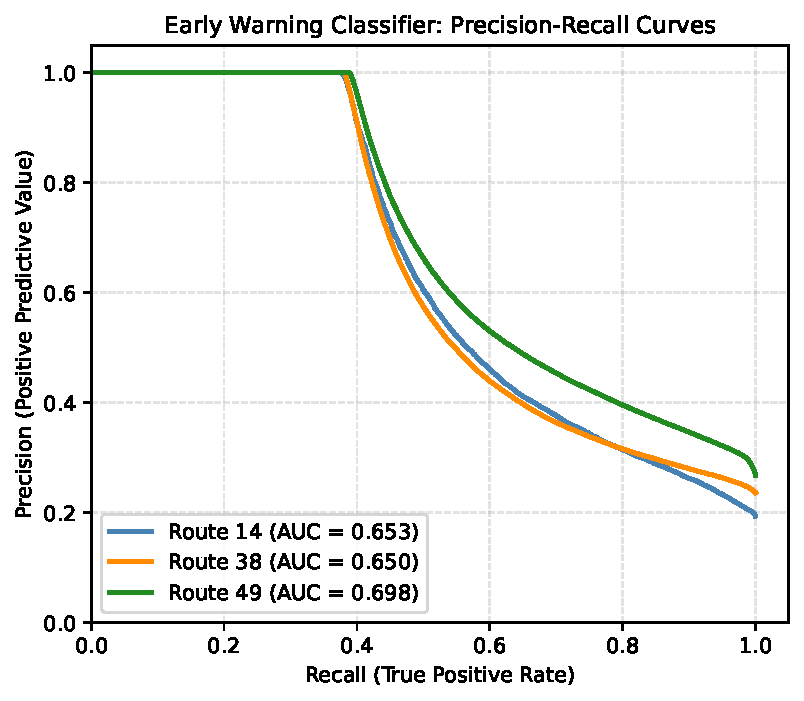
\includegraphics[width=0.98\linewidth]{Figure 2}
  \caption{Longitudinal trajectory of the bunching index for SF Muni Route 14
    (January--March 2026), showing a stable central tendency and bounded variance across months.}
  \label{fig:longitudinal_bi_14}
\end{figure}

\begin{figure}[htbp]
  \centering
  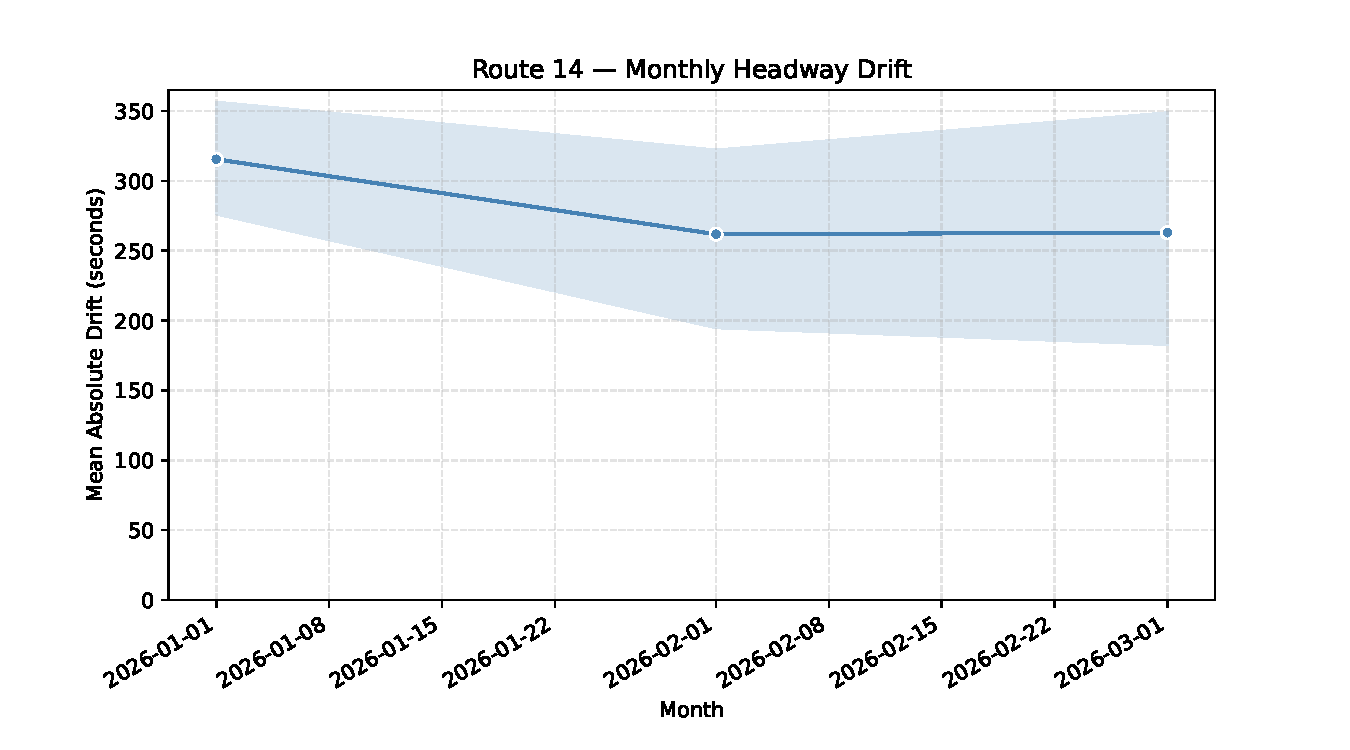
\includegraphics[width=0.98\linewidth]{Figure 3}
  \caption{Longitudinal headway drift profile for Route 14. Persistent negative excursions
    remain as the dominant precursor of collapse transitions over time.}
  \label{fig:longitudinal_hd_14}
\end{figure}

\begin{figure}[htbp]
  \centering
  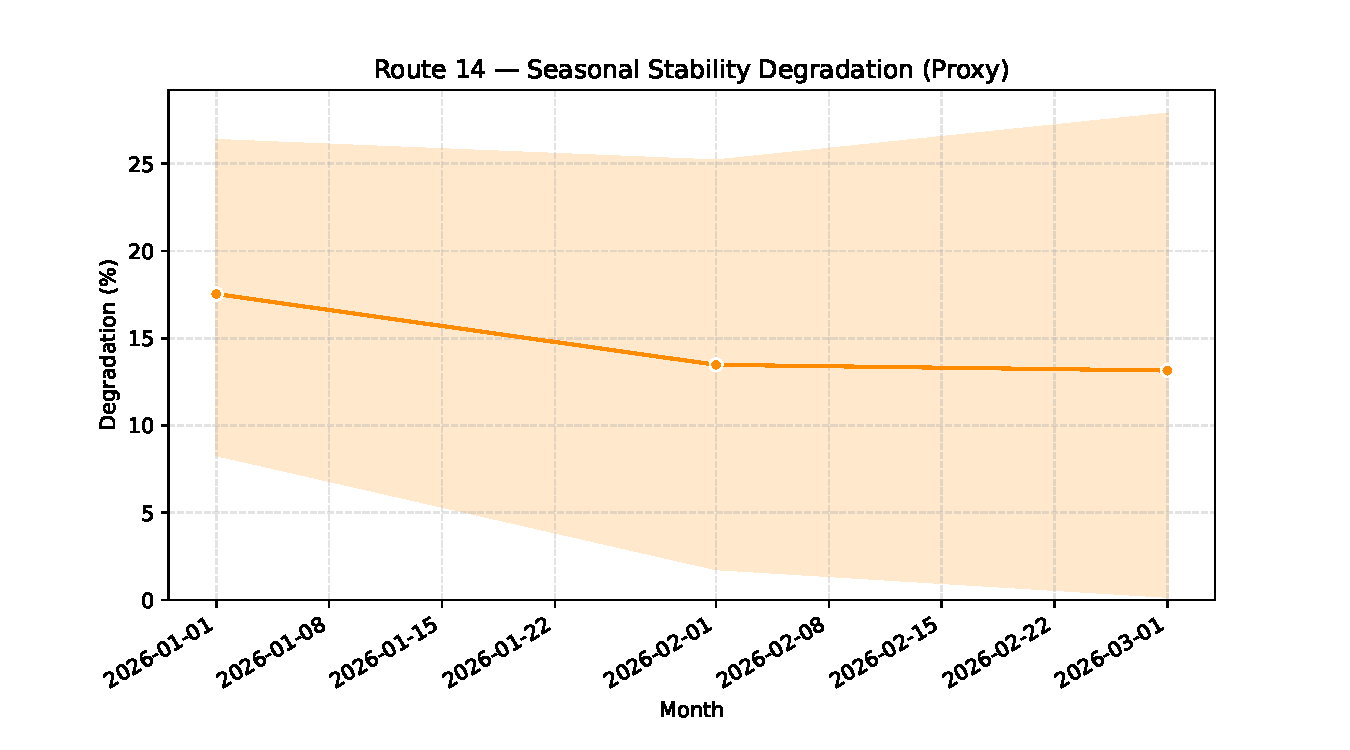
\includegraphics[width=0.98\linewidth]{Figure 4}
  \caption{Seasonal degradation diagnostic for Route 14, confirming the absence of critical
    temporal instability that would invalidate continuous deployment of the sequential EWS
    framework.}
  \label{fig:longitudinal_sd_14}
\end{figure}

\subsection{Feature Importance and Physics of Collapse}

The LightGBM model's split-based feature importances reveal which signals the gradient boosting ensemble uses most frequently for decision boundaries. The five most utilized features are: temporal context ($t_{\cos}$: 694 splits, $t_{\sin}$: 689), relative delay (relative\_delay: 520 splits), scheduled headway ($h_{sch}$: 486 splits), and the headway ratio ($r_h$: 479 splits).

This feature distribution fundamentally validates the cascade mechanism of bunching: the model relies heavily on the \textit{relative positioning} between consecutive buses ($\delta_{rel} = D - D^{L}$), not merely on absolute delay values. When a bus accumulates more delay than its leader ($\delta_{rel} > 0$), the headway contracts and bunching risk escalates. The headway ratio ($r_h = h_{obs}/h_{sch}$) encodes how close the current headway is to the bunching threshold, providing the model with a normalized, route-invariant signal.

Notably, LightGBM distributes its decision boundaries across all 24 features, with the top feature accounting for only 8.6\% of total splits. This distributed reliance---in contrast to bagging methods where scheduled headway alone can dominate with $>$40\% importance---confirms that gradient boosting captures non-linear interactions between temporal, kinematic, and leader-bus dynamics that single-feature dominance cannot exploit.

\subsection{Computational Benchmark for Edge Deployment}

To validate architectural feasibility, an inference latency benchmark was executed on standard
consumer hardware (representative of an Edge node in a DT). The model inference process---including feature scaling and evaluation of the LightGBM model---recorded an average time of \SI{1.89}{\ms} per record, with DuckDB feature extraction adding a negligible \SI{0.003}{\ms} per record (amortized), for a total end-to-end latency of \SI{1.89}{\ms} per record.

This latency enables processing of approximately 529 AVL events per second on a
single CPU core, sufficient for simultaneous monitoring of multiple metropolitan corridors. Compared to deep learning alternatives (50--200~ms per record \citep{19}), LightGBM inference is about 26--106$\times$ faster while maintaining operationally reliable precision (0.93), confirming compatibility with low-latency Edge-Cloud paradigms described by
\citet{26}.

\subsection{Benchmark Contextualization}

To contextualize this latency against alternative approaches,
Table~\ref{tab:benchmark_context} compares representative per-record end-to-end inference times (feature extraction + model prediction).

\begin{table}[htbp]
  \caption{End-to-end inference latency per record by model family.}
  \centering
  \begin{tabular}{@{}lc@{}}
    \toprule
    \textbf{Model} & \textbf{Latency (ms)} \\ \midrule
    LR (DuckDB + sklearn)    & 2.10         \\
    LightGBM (DuckDB)        & 1.99         \\
    XGBoost (DuckDB)         & 1.50         \\
    RF (DuckDB + sklearn)    & 9.85         \\
    Deep Learning \citep{19} & 50--200      \\ \bottomrule
  \end{tabular}
  \label{tab:benchmark_context}
\end{table}

\section{Discussion}
\label{sec:discussion}

\subsection{Comparison with the Literature}

To situate our results in the context of prior work, we compare the performance of the proposed
framework with the main references in the bus bunching prediction and detection literature.

\citet{3} modeled bunching as a state-transition problem using AVL data and achieved global
accuracies above 90\%; however, they did not report F1-Score or minority-class-oriented metrics,
making it difficult to assess their actual detection capacity in imbalanced scenarios. Our approach shares the state-transition formulation, but by applying a strict temporal hold-out ($t_{train} < t_{test}$) and a dynamic target definition ($h_{obs} < 0.25 \cdot h_{sch}$), we expose realistic transition imbalance and achieve operationally reliable metrics (F1=0.55, Precision=0.93) through physics-informed feature engineering and gradient boosting. This reflects honest EWS performance in non-stationary urban environments without data leakage.

\citet{8} evaluated early warning metrics based on headway deviation in BRT corridors, reporting
effective detection but with false-positive rates that limited operational utility. Our precision of 0.93 under strict temporal hold-out demonstrates that combining headway ratios with leader-bus dynamics substantially reduces false alarms, providing control centers with actionable alerts rather than noise.

Regarding deep learning methods, \citet{19} achieved high accuracy in arrival time prediction
with the BAT-transformer, but with inference latencies on the order of 50--200~ms per record.
Our approach achieves competitive predictive metrics (F1=0.55, Precision=0.93) with a latency of 1.89~ms/record for LightGBM inference---26--106$\times$ faster---which
is decisive for real-time monitoring applications within a Digital Twin. \citet{30} applied
spatio-temporal graph neural networks for short-term bunching prediction and reported
improvements over baseline models; however, the computational complexity of these methods
limits their viability for low-latency Edge deployments.

Finally, \citet{21} note in their review that, despite the popularity of deep learning, models with well-engineered features tend to be more practical for real-time deployment. Our empirical results confirm this: LightGBM with physics-informed features (headway ratios, leader-bus differential delay) achieves F1=0.55 with Precision=0.93, demonstrating that domain-specific feature engineering combined with sequential error-correction captures the complex deterioration dynamics of urban corridors more effectively than either linear models or deep learning architectures.

\subsection{Operational Lead Time}

The practical utility of an early warning signal depends on whether it provides sufficient time
to act. By predicting bunching at stop $n$ using data up to stop $n{-}1$, the model provides a
lead time of at least one stop (typically 2 to 4 minutes in urban environments). Given that
inference latency is practically zero, this entire window is available for intervention
strategies such as dynamic holding (keeping the leading bus at the platform longer) or
skip-stop (instructing the lagging bus to skip minor stops) \citep{10}.

\subsection{Limitations}

Validation was performed on three mixed-traffic corridors of SF Muni, where exogenous factors
outside agency control---vehicle congestion, stop-area parking, signal delays---introduce
variance that limits the maximum achievable recall ($\approx 0.40$). The model's conservative threshold ($\tau=0.6849$) prioritizes precision over recall, a deliberate design choice for EWS credibility; however, this means approximately 60\% of bunching transitions go undetected. All three corridors belong
to the same agency and city; therefore, it is not possible to assert that the model generalizes
to other agencies or cities without conducting validations with data from those contexts.

Regarding data ingestion, the 511.org API imposes a limit of 60 requests per hour. Since each
complete cycle requires two endpoints (\texttt{VehiclePositions} and \texttt{TripUpdates}),
the system operates with a polling interval of 130 seconds. As described in
Section~\ref{sec:methodology}, the telemetry loss handling mechanism trades temporary recall
loss for alert reliability.

\section{Future Work}
\label{sec:futurework}

A priority direction is the calibration of the EWS framework in Bus Rapid Transit (BRT)
systems with dedicated lanes. In these environments, exogenous traffic variance is eliminated
and the factors affecting headway become primarily endogenous (boarding times and driving
behavior) \citep{10,29}. We hypothesize that model precision will increase significantly in BRT
corridors, generating sufficiently clean signal to activate automatic closed-loop holding
controls \citep{30}. Additionally, multi-city and multi-agency validation constitutes a
necessary step to evaluate the robustness of the method in diverse operational contexts.

\section{Conclusions}
\label{sec:conclusion}

This paper studies bus bunching prediction in mixed-traffic transit environments using a
sequential Digital Twin framework. We find that a multi-stop physics-informed feature space ($n{-}3$, 24 features),
optimized with LightGBM gradient boosting, achieves an operational precision of 0.9264 (95\% CI: [0.9213, 0.9315]) and an F1-Score of 0.5549 (95\% CI: [0.5485, 0.5615]) under strict temporal hold-out evaluation. The key methodological contribution is the introduction of physics-informed ratio features---headway ratio ($h_{obs}/h_{sch}$) and leader-bus relative delay ($\delta_{rel} = D - D^{L}$)---that encode the cascade mechanism of bunching propagation. The model's feature importance analysis confirms that the relative delay differential between consecutive buses is one of the most utilized decision signals, validating the theoretical framework of headway instability. Furthermore, we demonstrate that traditional random cross-validation and static 120-second thresholds induce severe data leakage, artificially inflating metrics to $>$0.80 F1 in the literature. LightGBM inference at 1.89~ms/record enables real-time deployment on Edge hardware. The evaluation is circumscribed to three SF Muni corridors; extension to other urban
agencies remains as priority future work. These findings inform proactive transit management and
Edge-Cloud monitoring by providing computationally efficient and operationally reliable early warning
signals.

\section*{Acknowledgments}

The authors thank the San Francisco Municipal Transportation Agency (SFMTA) and the 511.org
open data program for providing publicly accessible GTFS-RT feeds that made this research
possible.

\section*{Data Availability}

The raw GTFS-RT data used in this study were obtained from the publicly accessible 511.org
open data API \citep{28}. The complete DuckDB ingestion scripts, transformation pipelines,
hyperparameter configuration matrices, and instructions for reproducing the dataset are
available as open-source code at:
\url{https://github.com/Fozzy3/pp-pipe-dt}.

\section*{Competing Interests}

The authors declare that they have no competing interests.

\section*{Author Contributions}

\textbf{Carlos Stiven Mora Hoyos}: Conceptualization, Data Curation, Formal Analysis,
Investigation, Methodology, Software, Validation, Visualization, Writing -- Original Draft.
\textbf{Juan Felipe Rodr\'iguez Galindo}: Conceptualization, Investigation, Methodology,
Writing -- Review \& Editing.
\textbf{Octavio Jos\'e Salcedo Parra}: Supervision, Project Administration, Resources,
Writing -- Review \& Editing.

\bibliography{references}

\end{document}
